% Set up the document
\documentclass{article}

% Page size
\usepackage[
    letterpaper,]{geometry}

% Lines between paragraphs
\setlength{\parskip}{\baselineskip}
\setlength{\parindent}{0pt}

% Math
\usepackage{mathtools}
\usepackage{amssymb}
\usepackage{commath}

% Math notation macros
\def\*#1{\mathbf{#1}}
\newcommand{\B}{\mathcal{B}}
\newcommand{\rhat}{\mathbf{\hat{r}}}
\newcommand{\thetahat}{\boldsymbol{\hat{\theta}}}
\newcommand{\zhat}{\mathbf{\hat{z}}}
\newcommand{\dadvd}[2]{\dfrac{\text{D} #1}{\text{D} #2}} % advective derivative

% Links
\usepackage{hyperref}

% Page numbers at top right
\usepackage{fancyhdr}
\pagestyle{fancy}
\fancyhf{}
\fancyhead[R]{\thepage}
\renewcommand\headrulewidth{0pt}

% Graphics
\usepackage{float}
\usepackage{graphicx}
\graphicspath{ {./img/} }

\begin{document}

\textbf{MATH 462 Homework 2} \\
\textbf{Matt Wiens \#301294492} \\
\textbf{2020-01-29}

\textbf{C) Lagrangian Derivation of Continuity.} Another common
derivation of the fluid equations relies on the integral identities of
multi-variable calculus---instead of the infinitesimal control volume
approach shown in lectures. Present a Lagrangian derivation of the
continuity equation based on the ideas and notation sketched out below.
Organize your write-up as a numbers list identifying each of the major
concepts/steps.

Consider any initial blob of fluid, $\B(0)$, and let $\B(t)$ Be the blob
of this original fluid as it moves with the flow. Note that we assume
the flow velocity is continuous so that we do not have to be concerned
with the fluid blob breaking into multiple bloblets.

Define the total fluid mass inside the blob by the volume integral over
the space occupied by the blob
%
\begin{equation*}
    M(t) = \iiint_{\B(t)} \rho(\*x, t) \dif x \dif y \dif z
\end{equation*}
%
and then explain how the principle of conservation of mass requires
%
\begin{equation*}
    \dod{M}{t} = 0
    .
\end{equation*}
%
Taking the derivative of the integral formula for $M(t)$ involves two
contributions: time-variations in the integrand $\rho(\*x, t)$, and
motion of the blob $\B(t)$. This differentiation is essentially a
three-dimensional version of Leibniz's rule. In particular, explain
explicitly how the second contribution can be expressed as a surface
integral. The basic idea is that over a time-interval $\Delta t$ the
change to the blob geometry can be accounted for by summing over the
displacements of small surface patches $\Delta S$. This surface integral
can be then converted to a volume integral using the divergence theorem.
Finally, invoke the zero-integrand property which states that if an
integral of the form
%
\begin{equation*}
    \iiint_{\B(t)} \cbr{\text{integrand}} \dif x \dif y \dif z = 0
\end{equation*}
%
for \textit{all} choices of $\B(t)$, then the integrand must be zero
everywhere.

\textbf{Solution}

Consider a blob of fluid $\B(t)$ that moves with some continuous flow
$\*U(\*x, t)$, and where the density of the entire fluid is given by
$\rho(\*x, t)$.

1. Define the mass inside of the blob at any time $t$ to be
%
\begin{equation*}
    M(t) \coloneqq \iiint_{\B(t)} \rho(\*x, t) \dif \*x
    .
\end{equation*}

2. Since we are dealing with a blob of fluid (as opposed to a fixed volume
in space in the Eulerian case), we are fixing the mass inside the fluid,
and hence we have
%
\begin{equation}
    \dod{M}{t} = 0
    .
    \label{eq:c-cons-mass}
\end{equation}

3. Changes in mass can happen because of two reasons: (a) changes in the
density of the fluid contained in the blob, which can be expressed as
%
\begin{equation*}
    \iiint_{\B(t)} \dpd{\rho}{t} \dif V
    ;
\end{equation*}
%
and (b) changes due to fluid entering and leaving the surface of blob as
it moves through space. The change in mass entering and leaving for any
small surface element $\dif S$ is $(\*U \cdot \*n) \rho \dif S$, where
$\*n$ is the outer normal vector to the surface of $\B(t)$. Thus
integrating over the surface we have the net mass leaving the surface:
%
\begin{equation*}
    \iint_{\partial \B(t)} (\*U \cdot \*n) \rho \dif S
    .
\end{equation*}
%
Combining these two contributions and using~\eqref{eq:c-cons-mass}, we have
%
\begin{equation*}
    \iiint_{\B(t)} \dpd{\rho}{t} \dif V
    +
    \iint_{\partial \B(t)} (\*U \cdot \*n) \rho \dif S
    = 0
    .
\end{equation*}

4. Using the divergence theorem, we can express the above equation purely
in terms of a volume integral:
%
\begin{equation*}
    \iiint_{\B(t)}
        \dpd{\rho}{t}
        +
        \nabla \cdot (\rho \*U)
    \dif V
    = 0
    .
\end{equation*}

5. Since $\B$ was an arbitrary fluid blob, it must hold that the integrand
\textit{always} vanishes, and hence we have that
%
\begin{equation}
    \dpd{\rho}{t}
    +
    \nabla \cdot (\rho \*U)
    = 0
    .
    \label{c:zero-integrand}
\end{equation}
%
We can put the left-hand side of \eqref{c:zero-integrand} in a more
familiar form as follows:
%
\begin{align*}
    \dpd{\rho}{t} + \nabla \cdot (\rho \*U) = 0
        = \dpd{\rho}{t} + \nabla \rho \cdot \*U + \rho (\nabla \cdot \*U)
        = \dadvd{\rho}{t} + \rho (\nabla \cdot \*U)
    .
\end{align*}
%
This leaves us with the familiar conservation of mass equation
%
\begin{equation*}
    \dadvd{\rho}{t} + \rho (\nabla \cdot \*U) = 0
    .
\end{equation*}

\newpage

\textbf{D) Polar Coordinates Again.} Present a control volume derivation
of the PDE representing Newton's law in fully three-dimensional cylindrical
coordinates $(r, \theta, z)$. Define the velocity as
%
\begin{equation*}
    \*U(r, \theta, z, t)
        = U(r, \theta, z, t) \rhat
          + V(r, \theta, z, t) \thetahat
          + W(r, \theta, z, t) \zhat
          ;
\end{equation*}
%
you are reminded that the $\rhat$ and $\thetahat$-directions are
functions of $\theta$. Present your results in acceleration form.

\textbf{Solution}

Consider the control volume shown in Figure~\ref{figure:d-cv}. We want
to determine the PDE that results from Newton's law:
%
\begin{equation*}
    \parbox[t]{13em}{\centering
        net change of momentum inside $\Delta V$ from $t \to t + \Delta t$
    }
    +
    \parbox[t]{13em}{\centering
        momentum leaving $\Delta V$
    }
    =
    \parbox[t]{5em}{\centering
        applied force
    }
    \times
    \Delta t
    .
\end{equation*}
%
Now, the total momentum of the control volume is given by
%
\begin{equation*}
    \iiint_{\Delta V} \rho(\*x, t) \*U(\*x, t) \dif \*x
\end{equation*}
%
and, given that $\Delta V$ is small, can thus be approximated by
%
\begin{equation*}
    \rho(\*x, t) \*U(\*x, t) \Delta V
    .
\end{equation*}
%
Using this approximation we can determine the net change in momentum
from time $t$ to $t + \Delta t$ with
%
\begin{align*}
    \del{
        \rho(\*x, t + \Delta t ) \*U(\*x, t + \Delta t )
        - \rho(\*x, t) \*U(\*x, t)
    } \Delta V
    &= \frac{
        \rho(\*x, t + \Delta t ) \*U(\*x, t + \Delta t )
        - \rho(\*x, t) \*U(\*x, t)
    }{\Delta t} \Delta V \Delta t \\
    &\approx \dpd{\del{\rho \*U}}{t} \Delta V \Delta t
    .
\end{align*}
%
Now let's consider the momentum leaving the control volume during the
$\Delta t$ time window. Consider the change in momentum in the
$\thetahat$ direction (see Figure~\ref{figure:d-theta}):
%
\begin{align*}
    &
    \del{
        \rho(r, \theta + \Delta \theta, z, t)
        \*U(r, \theta + \Delta \theta, z, t)
        V(r, \theta + \Delta \theta, z, t)
        - \rho(r, \theta, z, t)
        \*U(r, \theta, z, t)
        V(r, \theta, z, t)
    } \Delta t \Delta r \Delta z \\[0.5ex]
    &=
    \frac{
        \rho(r, \theta + \Delta \theta, z, t)
        \*U(r, \theta + \Delta \theta, z, t)
        V(r, \theta + \Delta \theta, z, t)
        - \rho(r, \theta, z, t)
        \*U(r, \theta, z, t)
        V(r, \theta, z, t)
    }{\Delta \theta}
    \frac{\Delta t \Delta V}{r} \\
    &\approx
    \frac{1}{r} \dpd{\del{\rho \*U V}}{\theta} \Delta t \Delta V
    .
\end{align*}
%
\begin{figure}[b]
    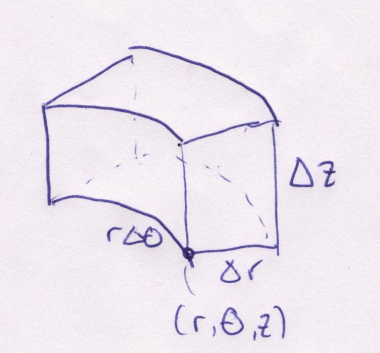
\includegraphics[width=8em]{d-cv}
    \centering
    \caption{The control volume}
    \label{figure:d-cv}
\end{figure}
%
\begin{figure}[!ht]
    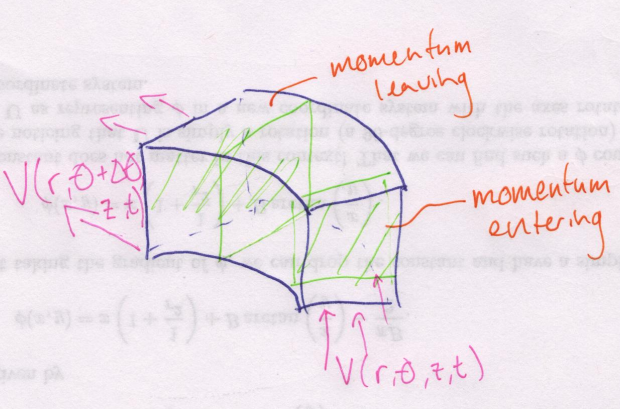
\includegraphics[width=15.2em]{d-theta}
    \centering
    \caption{Momentum change in $\thetahat$ direction}
    \label{figure:d-theta}
\end{figure}
%
\begin{figure}[!ht]
    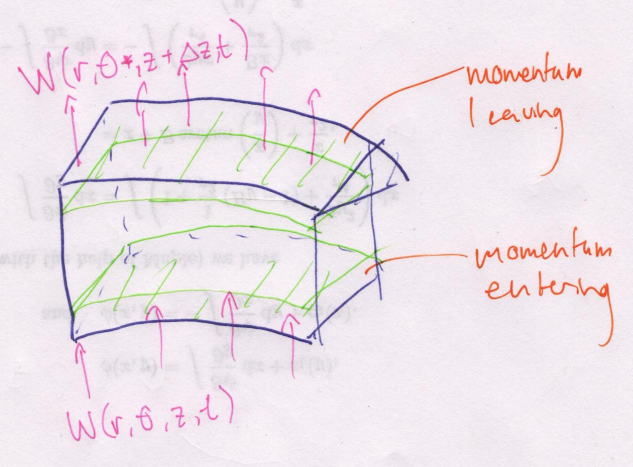
\includegraphics[width=15.2em]{d-z}
    \centering
    \caption{Momentum change in $\zhat$ direction}
    \label{figure:d-z}
\end{figure}
%
We'll now consider the momentum leaving in the $\zhat$ direction (see
Figure~\ref{figure:d-z}). Note that the area of the ``top'' (and bottom) of the control
volume is
%
\begin{align*}
    &\frac{1}{2}
    \del{r \Delta \theta + (r + \Delta r) \Delta \theta}
    \sqrt{(\Delta r)^2 - \frac{1}{4}
        \del{r \Delta \theta - (r + \Delta r) \Delta \theta}^2
    } \\
    &=
    \frac{1}{2}
    \del{2 r \Delta \theta + \Delta r \Delta \theta}
    \sqrt{(\Delta r)^2 - \frac{1}{4}
        \del{\Delta r \Delta \theta}^2
    } \\
    &\approx r \Delta r \Delta \theta
    ,
\end{align*}
%
where in the last step we discarded $\mathcal{O}(\Delta^3)$ terms.
Therefore, the change in momentum in the $\zhat$ direction is
approximately
%
\begin{align*}
    &
    \del{
        \rho(r, \theta, z + \Delta z, t)
        \*U(r, \theta, z + \Delta z, t)
        W(r, \theta, z + \Delta z, t)
        - \rho(r, \theta, z, t)
        \*U(r, \theta, z, t)
        W(r, \theta, z, t)
    } r \Delta r \Delta \theta \Delta t \\[0.5ex]
    &=
    \frac{
        \rho(r, \theta, z + \Delta z, t)
        \*U(r, \theta, z + \Delta z, t)
        W(r, \theta, z + \Delta z, t)
        - \rho(r, \theta, z, t)
        \*U(r, \theta, z, t)
        W(r, \theta, z, t)
    }{\Delta z} \Delta V \Delta t \\
    &\approx \dpd{\del{\rho \*U W}}{z} \Delta V \Delta t
    .
\end{align*}
%
Finally, we'll calculate the change in momentum in the $\rhat$
direction, with the aid of Figure~\ref{figure:d-r}:
%
\begin{align*}
    &
    \del{
        \rho(r + \Delta r, \theta, z, t)
        \*U(r + \Delta r, \theta, z, t)
        U(r + \Delta r , \theta, z, t)
        (r + \Delta r)
        - \rho(r, \theta, z, t)
        \*U(r, \theta, z, t)
        U(r, \theta, z, t)
        r
    }
    \\
    &\qquad \quad \cdot \Delta r \Delta \theta \Delta t
    \\
    &=
    \frac{
        \rho(r + \Delta r, \theta, z, t)
        \*U(r + \Delta r, \theta, z, t)
        U(r + \Delta r , \theta, z, t)
        (r + \Delta r)
        - \rho(r, \theta, z, t)
        \*U(r, \theta, z, t)
        U(r, \theta, z, t)
        r
    }{\Delta r}
    \\
    &\qquad \quad \cdot \frac{\Delta V \Delta t}{r}
    \\[0.5ex]
    &\approx \frac{1}{r} \dpd{\del{\rho \*U U r}}{r} \Delta V \Delta t
    .
\end{align*}
%
\begin{figure}[!ht]
    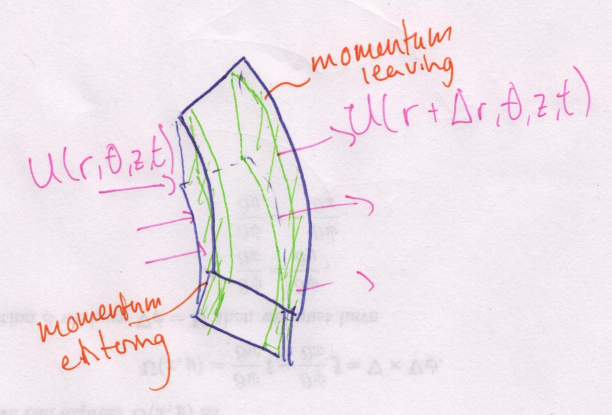
\includegraphics[width=15.2em]{d-r}
    \centering
    \caption{Momentum change in $\rhat$ direction}
    \label{figure:d-r}
\end{figure}
%
Now we can express the left-hand side of Newton's law in cylindrical
coordinates:
%
\begin{equation}
    \dpd{\del{\rho \*U}}{t} \Delta V \Delta t
    + \frac{1}{r} \dpd{\del{\rho \*U U r}}{r} \Delta V \Delta t
    + \frac{1}{r} \dpd{\del{\rho \*U V}}{\theta} \Delta t \Delta V
    + \dpd{\del{\rho \*U W}}{z} \Delta V \Delta t
    .
    \label{eq:d-newton-lhs}
\end{equation}
%
We can simplify this expression by using the conservation of mass
equation:
%
\begin{equation*}
    \dpd{\rho}{t}
        + \frac{1}{r} \dpd{\del{\rho U r}}{r}
        + \frac{1}{r} \dpd{\del{\rho V}}{\theta}
        + \dpd{\del{\rho W}}{z}
        = 0
        .
\end{equation*}
%
Thus we can simplify~\eqref{eq:d-newton-lhs} as follows (to simplify
these steps, I'll omit the $\Delta V \Delta t$ terms below):
%
\begin{align*}
    &\dpd{\del{\rho \*U}}{t}
    + \frac{1}{r} \dpd{\del{\rho \*U U r}}{r}
    + \frac{1}{r} \dpd{\del{\rho \*U V}}{\theta}
    + \dpd{\del{\rho \*U W}}{z}
    \\
    &=
    \*U \dpd{\rho}{t}
    + \rho \dpd{\*U}{t}
    + \frac{1}{r} \*U \dpd{\del{\rho U r}}{r}
    + \rho U \dpd{\*U}{r}
    + \frac{1}{r} \*U \dpd{\del{\rho V}}{\theta}
    + \frac{1}{r} \rho V \dpd{\*U}{\theta}
    + \*U \dpd{\del{\rho W}}{z}
    + \rho W \dpd{\*U}{z}
    \\
    &=
    \rho \dpd{\*U}{t}
    + \rho U \dpd{\*U}{r}
    + \frac{1}{r} \rho V \dpd{\*U}{\theta}
    + \rho W \dpd{\*U}{z}
    + \*U \del{
        \dpd{\rho}{t}
        + \frac{1}{r} \dpd{\del{\rho U r}}{r}
        + \frac{1}{r} \dpd{\del{\rho V}}{\theta}
        + \dpd{\del{\rho W}}{z}
    }
    \\
    &=
    \rho \dpd{\*U}{t}
    + \rho U \dpd{\*U}{r}
    + \frac{1}{r} \rho V \dpd{\*U}{\theta}
    + \rho W \dpd{\*U}{z}
    .
\end{align*}
%
Let's complete the expression of Newton's law in cylindrical coordinates
by considering the applied forces. It turns out we don't need to do
anything different than in the Cartesian coordinate derivation, since
both coordinate systems share the $z$-coordinate (which gravity acts
along) and because the gradient operator is ``coordinate-free'' (so we
can write pressure just as in the Cartesian case). Hence our applied
forces are simply given by
%
\begin{equation*}
    \del{- \nabla p - \rho g \zhat} \Delta V
    .
\end{equation*}
%
Thus Newton's law in cylindrical coordinates is
%
\begin{equation*}
    \del{
        \rho \dpd{\*U}{t}
        + \rho U \dpd{\*U}{r}
        + \frac{1}{r} \rho V \dpd{\*U}{\theta}
        + \rho W \dpd{\*U}{z}
    } \Delta V \Delta t
    =
    \del{- \nabla p - \rho g \zhat} \Delta V \Delta t
    ,
\end{equation*}
%
or, in ``acceleration form'',
%
\begin{equation*}
    \dpd{\*U}{t}
    + U \dpd{\*U}{r}
    + \frac{1}{r} V \dpd{\*U}{\theta}
    + W \dpd{\*U}{z}
    =
    - \frac{1}{\rho} \nabla p - g \zhat
    .
\end{equation*}
%
This is a vector equation. First, note that in cylindrical coordinates,
the advective derivative is given by
%
\begin{align*}
    \dadvd{\psi}{t}
        &= \dpd{\psi}{t} + \*U \cdot \nabla \psi \\
        &= \dpd{\psi}{t} + \*U \cdot
            \del{
                \dpd{\psi}{r},
                \frac{1}{r} \dpd{\psi}{\theta},
                \dpd{\psi}{z}
            } \\
        &=
            \dpd{\psi}{t}
            + U \dpd{\psi}{r}
            + V \frac{1}{r} \dpd{\psi}{\theta}
            + W \dpd{\psi}{z}
        .
\end{align*}
%
Let's break up our Newton's law equation in terms of components.
First, we'll evaluate the vector derivatives:
%
\begin{align*}
    \dpd{\*U}{t} &= \dpd{U}{t} \rhat + \dpd{V}{t} \thetahat + \dpd{W}{t} \zhat, \\
    \dpd{\*U}{r}
        &= \dpd{U}{r} \rhat
            + \dpd{V}{r} \thetahat
            + \dpd{W}{r} \zhat
    ,
    \\
    \dpd{\*U}{\theta}
        &= \dpd{U}{\theta} \rhat
            + U \thetahat
            + \dpd{V}{r} \thetahat
            - V \rhat
            + \dpd{W}{r} \zhat
    ,
    \\
    \dpd{\*U}{z} &= \dpd{U}{z} \rhat + \dpd{V}{z} \thetahat + \dpd{W}{z} \zhat
    .
\end{align*}
%
Thus in the $r$ component, Newton's the acceleration form is
%
\begin{align*}
    &\dpd{U}{t}
    + U \dpd{U}{r}
    + \frac{1}{r} V \del{\dpd{U}{\theta} - V}
    + W \dpd{U}{z}
    =
    - \frac{1}{\rho} \dpd{p}{r}
    \\
    &\implies
    \dadvd{U}{t} - \frac{V^2}{r}
    =
    - \frac{1}{\rho} \dpd{p}{r}
    ;
\end{align*}
%
and in the $\theta$ component,
%
\begin{align*}
    &\dpd{V}{t}
    + U \dpd{V}{r}
    + \frac{1}{r} V \del{\dpd{V}{\theta} + U}
    + W \dpd{U}{z}
    =
    - \frac{1}{\rho} \frac{1}{r} \dpd{p}{\theta}
    \\
    &\implies
    \dadvd{V}{t} + \frac{U V}{r}
    =
    - \frac{1}{\rho} \frac{1}{r} \dpd{p}{\theta}
    ;
\end{align*}
%
and in the $z$ component,
%
\begin{align*}
    &\dpd{W}{t}
    + U \dpd{W}{r}
    + \frac{1}{r} V \dpd{W}{\theta}
    + W \dpd{W}{z}
    =
    - \frac{1}{\rho} \dpd{p}{r} - g
    \\
    &\implies
    \dadvd{W}{t}
    =
    - \frac{1}{\rho} \dpd{p}{z} - g
    .
\end{align*}
%
Putting these together, we thus have
%
\begin{equation*}
    \dadvd{\*U}{t} - \frac{V^2}{r} \rhat + \frac{U V}{r} \thetahat
        = - \frac{1}{\rho} \nabla p - g \zhat
    .
\end{equation*}

\end{document}
